% Drawing 144/03-5 -- folder 144, batch 03, archive page 55 (PDF page 56).
% Transcription: Un graphe (arbre) en traits gras épaissis, entouré d'un contour fin qui en dessine le voisinage (le disque $D(X/K)$) ; sommets marqués en gras, quelques points sur le bord. Une flèche désigne une extrémité : \og arête repliée \fg, avec le petit croquis d'un \og modèle intuitif \fg{} (un Y épaissi dont une branche est repliée sur elle-même).
% Kind: thickened tree (disc D(X/K)) and folded-edge model. Method 2 (schematic redraw from the facsimile). Status: ok.
% Notes: The tree in thickened bold strokes, its outline (thin contour) drawn as one closed curve; vertices as dots. Right: the small thickened Y with one branch folded on itself ("modele intuitif"), pointed to by "<- arete repliee". The surrounding legend is text and is not drawn.
% Coordinates: 1 unit = 1 mm = 1/100 of the crop width (bbox in page fractions: [0.3, 0.5, 0.6, 0.62]).
% Redrawn by Claude (claude-opus-5-5), issue #73, 2026-11-07; not checked by a human; not compiled (no TeX in the session).
% Rights: reproduces part of the work -- behind RENDER_TRANSCRIPTS, never published by itself.
\documentclass[tikz,border=3pt]{standalone}
\usepackage{amsmath,amssymb}
\usetikzlibrary{patterns,arrows.meta}
\tikzset{pencil/.style={black!45}, struck/.style={black!35}, mark/.style={circle,draw,inner sep=1.3pt}, pt/.style={circle,fill,inner sep=0.9pt}, opt/.style={circle,draw,fill=white,inner sep=1.1pt}}
\begin{document}
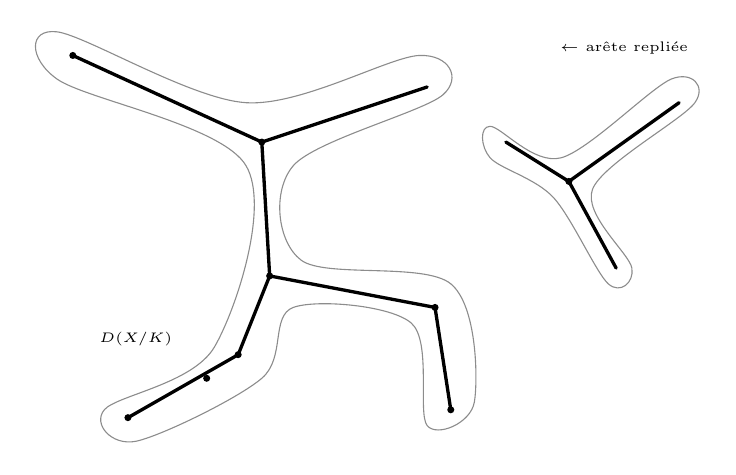
\begin{tikzpicture}[x=1mm,y=1mm,line cap=round,line join=round,font=\scriptsize]
\draw[very thick] (18,-16) -- (42,-27) -- (63,-20);
\draw[very thick] (42,-27) -- (43,-44) -- (64,-48) -- (66,-61);
\draw[very thick] (43,-44) -- (39,-54) -- (25,-62);
\node[pt] at (18,-16) {};
\node[pt] at (42,-27) {};
\node[pt] at (43,-44) {};
\node[pt] at (64,-48) {};
\node[pt] at (66,-61) {};
\node[pt] at (39,-54) {};
\node[pt] at (25,-62) {};
\node[pt] at (35,-57) {};
\draw[pencil] plot[smooth cycle, tension=0.55] coordinates {(16,-13) (40,-22) (62,-16) (65,-21) (46,-30) (47,-42) (66,-45) (69,-60) (63,-63) (61,-50) (46,-48) (42,-57) (26,-65) (22,-61) (36,-53) (40,-30) (16,-19)};
\draw[very thick] (73,-27) -- (81,-32) -- (95,-22);
\draw[very thick] (81,-32) -- (87,-43);
\node[pt] at (81,-32) {};
\draw[pencil] plot[smooth cycle, tension=0.55] coordinates {(71,-25) (80,-29) (94,-19) (97,-22) (84,-33) (89,-43) (86,-45) (79,-34) (71,-29)};
\node[inner sep=1pt] at (26,-52) {\tiny $D(X/K)$};
\node[inner sep=1pt] at (88,-15) {\tiny $\leftarrow$ ar\^ete repli\'ee};
\end{tikzpicture}
\end{document}
